% MTL730 -- Formula Sheet / Short Notes (Lectures 2--8)
\documentclass[10pt,a4paper]{article}

\usepackage[margin=0.55in,top=0.5in,bottom=0.5in]{geometry}
\usepackage{amsmath,amssymb,mathtools}
\usepackage{tikz}
\usetikzlibrary{arrows.meta,positioning,shapes.geometric,fit,calc}
\usepackage[skins,breakable]{tcolorbox}
\usepackage{enumitem}
\usepackage{multicol}
\usepackage{microtype}
\usepackage{fancyhdr}
\usepackage{xcolor}

\pagestyle{fancy}
\fancyhf{}
\fancyhead[L]{\small\sffamily MTL730 --- Formula Sheet}
\fancyhead[R]{\small\sffamily Lectures 2--8}
\fancyfoot[C]{\small\thepage}
\renewcommand{\headrulewidth}{0.4pt}

\DeclareMathOperator{\gcdop}{gcd}
\DeclareMathOperator{\ord}{ord}
\DeclareMathOperator{\ind}{ind}
\DeclareMathOperator{\charp}{char}
\newcommand{\Z}{\mathbb Z}
\newcommand{\N}{\mathbb N}
\newcommand{\F}{\mathbb F}
\newcommand{\Fp}{\mathbb F_p}
\newcommand{\phiE}{\varphi}
\newcommand{\units}[1]{\bigl(\Z/#1\Z\bigr)^\times}

% palette
\definecolor{L2}{HTML}{1B4F72}
\definecolor{L3}{HTML}{0E6655}
\definecolor{L4}{HTML}{7B241C}
\definecolor{L5}{HTML}{6C3483}
\definecolor{L6}{HTML}{1A5276}
\definecolor{L7}{HTML}{B9770E}
\definecolor{L8}{HTML}{1C2833}
\definecolor{boxbg}{HTML}{F8F9F9}
\definecolor{mapbg}{HTML}{EBF5FB}

\tcbset{
  common/.style={
    enhanced, breakable, sharp corners=southwest,
    boxrule=0.6pt, left=4pt, right=4pt, top=3pt, bottom=3pt,
    fonttitle=\bfseries\sffamily\small, coltitle=white,
    colback=boxbg, before skip=5pt, after skip=5pt
  }
}

\newtcolorbox{lecbox}[2][]{
  common, colbacktitle=#2, colframe=#2, title={#1}
}

\newcommand{\one}[1]{\par\vspace{1pt}\noindent{\sffamily\bfseries\tiny\color{black!60}#1}\par\vspace{1pt}}
\newcommand{\note}[1]{\par\vspace{1pt}{\small\textit{#1}}\par}

\title{\vspace{-1.2em}\textbf{\sffamily MTL730 --- Formula Sheet}\\[1mm]
\large\sffamily Short Notes $\cdot$ Lectures 2--8 $\cdot$ Number Theory \& Finite Fields}
\author{}
\date{}

\begin{document}
\maketitle
\vspace{-1.6em}

% ============================================================
% MIND MAP
% ============================================================
\begin{center}
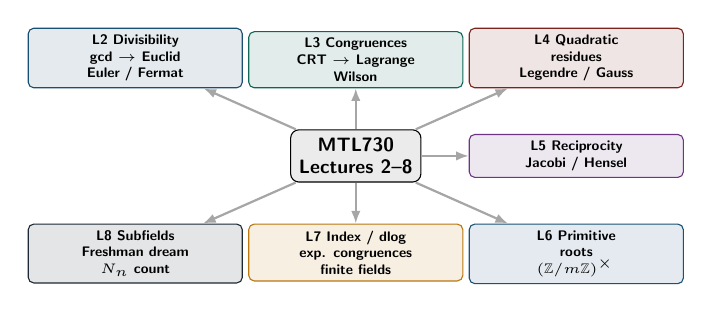
\begin{tikzpicture}[
  font=\sffamily\scriptsize,
  node distance=5.2mm and 6mm,
  box/.style={draw=#1, fill=#1!12, rounded corners=2pt, align=center,
              inner sep=2.4pt, text width=2.55cm, font=\sffamily\tiny\bfseries},
  hub/.style={draw=black, fill=black!8, rounded corners=3pt, align=center,
              inner sep=3pt, font=\sffamily\scriptsize\bfseries},
  arr/.style={-{Latex[length=1.6mm]}, thick, gray!70}
]
\node[hub] (C) {MTL730\\Lectures 2--8};

\node[box=L2, above left=of C] (A1) {L2 Divisibility\\gcd $\to$ Euclid\\Euler / Fermat};
\node[box=L3, above=of C] (A2) {L3 Congruences\\CRT $\to$ Lagrange\\Wilson};
\node[box=L4, above right=of C] (A3) {L4 Quadratic\\residues\\Legendre / Gauss};
\node[box=L5, right=of C] (A4) {L5 Reciprocity\\Jacobi / Hensel};
\node[box=L6, below right=of C] (A5) {L6 Primitive\\roots\\$(\Z/m\Z)^\times$};
\node[box=L7, below=of C] (A6) {L7 Index / dlog\\exp. congruences\\finite fields};
\node[box=L8, below left=of C] (A7) {L8 Subfields\\Freshman dream\\$N_n$ count};

\foreach \n in {A1,A2,A3,A4,A5,A6,A7}
  \draw[arr] (C) -- (\n);
\end{tikzpicture}
\end{center}

\vspace{-2mm}
{\centering\sffamily\tiny
\textcolor{L2}{\rule{1.1em}{0.7em} L2}\;
\textcolor{L3}{\rule{1.1em}{0.7em} L3}\;
\textcolor{L4}{\rule{1.1em}{0.7em} L4}\;
\textcolor{L5}{\rule{1.1em}{0.7em} L5}\;
\textcolor{L6}{\rule{1.1em}{0.7em} L6}\;
\textcolor{L7}{\rule{1.1em}{0.7em} L7}\;
\textcolor{L8}{\rule{1.1em}{0.7em} L8}
\par}

% ============================================================
\begin{lecbox}[Lecture 2 --- Divisibility, gcd, Euler, Fermat]{L2}

\one{DIVISIBILITY \& GCD}
\[
a\mid b \iff b=ac \quad(c\in\Z)
\qquad
d\mid a,\; d\mid b \;\Longrightarrow\; d\mid ax+by
\]
\[
\gcd(a,b)=\min\bigl\{d>0:d=ax+by,\;x,y\in\Z\bigr\}
\qquad
\gcd(0,0)=0
\]
\[
d=\gcd(a,b)\;\Longrightarrow\; \exists\,x,y:\; d=ax+by
\qquad\text{(B\'ezout)}
\]
\[
c=ax+by \;\Longrightarrow\; \gcd(a,b)\mid c
\qquad
\text{coprime}\iff \gcd(a,b)=1
\]

\one{DIVISION / EUCLIDEAN ALGORITHM}
\[
a=bq+r,\quad 0\le r<b
\qquad\text{(unique)}
\]
\[
a=qb+r \;\Longrightarrow\; \gcd(a,b)=\gcd(b,r)
\qquad
\text{last nonzero remainder}=\gcd(a,b)
\]

\one{PRIMES \& FTA}
\[
n=p_1^{e_1}\cdots p_k^{e_k}
\qquad\text{(unique, }e_i\ge1\text{)}
\]
\[
N=p_1\cdots p_n+1
\qquad
N\not\equiv 0\pmod{p_i}
\qquad\text{(Euclid: infinitely many primes)}
\]

\one{LINEAR DIOPHANTINE}
\[
ax+by=c
\text{ solvable in }\Z^2
\;\Longleftrightarrow\;
\gcd(a,b)\mid c
\]
If $(x_0,y_0)$ is one solution, all others differ by solutions of $ax+by=0$.

\one{CONGRUENCE}
\[
a\equiv b\pmod m \iff m\mid(a-b)
\]
\[
a\equiv b,\;c\equiv d \;\Longrightarrow\; ac\equiv bd,\;\; ax+cy\equiv bx+dy\pmod m
\]
\[
a\equiv b \;\Longrightarrow\; f(a)\equiv f(b)\pmod m
\qquad(f\in\Z[x])
\]
\[
ac\equiv bc\pmod m,\; d=\gcd(m,c)
\;\Longrightarrow\;
a\equiv b\pmod{m/d}
\]
\[
\gcd(m,c)=1 \;\Longrightarrow\; \text{cancel }c
\qquad
a\equiv b\pmod m \;\Longrightarrow\; \gcd(a,m)=\gcd(b,m)
\]
\[
\overline a=\{x:x\equiv a\pmod m\}
\qquad
\Z=\overline 0\cup\cdots\cup\overline{m-1}
\]

\one{RESIDUE SYSTEMS \& $\phi$}
\[
\phiE(m)=\#\{a:1\le a\le m,\;\gcd(a,m)=1\}
\]
CRS = one rep from each class. RRS = $\phiE(m)$ coprime, pairwise incongruent.
If $\gcd(k,m)=1$, multiplying a CRS/RRS by $k$ yields another.

\one{EULER / FERMAT / $\phi$ FORMULA}
\[
\gcd(a,m)=1 \;\Longrightarrow\; a^{\phiE(m)}\equiv 1\pmod m
\qquad\text{(Euler)}
\]
\[
p\text{ prime}\;\Longrightarrow\; a^p\equiv a\pmod p
\qquad
p\nmid a\;\Longrightarrow\; a^{p-1}\equiv 1\pmod p
\qquad\text{(Fermat)}
\]
\[
\phiE(p^e)=p^e-p^{e-1}=p^e\Bigl(1-\frac1p\Bigr)
\qquad
\gcd(m,n)=1\;\Longrightarrow\;\phiE(mn)=\phiE(m)\phiE(n)
\]
\[
\boxed{\displaystyle
\phiE(m)=m\prod_{p\mid m}\Bigl(1-\frac1p\Bigr)
}
\qquad
m=p_1^{e_1}\cdots p_r^{e_r}
\]
\end{lecbox}

% ============================================================
\begin{lecbox}[Lecture 3 --- Linear congruences, CRT, Lagrange, Wilson]{L3}

\one{LINEAR CONGRUENCE $ax\equiv b\pmod m$}
\[
\gcd(a,m)=1 \;\Longrightarrow\;
x\equiv a^{\phiE(m)-1}b\pmod m
\qquad\text{(unique)}
\]
\[
ax\equiv b\pmod m
\text{ solvable}
\;\Longleftrightarrow\;
d=\gcd(a,m)\mid b
\]
Then exactly $d$ solutions modulo $m$. Divide by $d$:
\[
\frac ad\,x\equiv\frac bd\pmod{\frac md}
\qquad
\gcd\!\Bigl(\tfrac ad,\tfrac md\Bigr)=1
\]
If $t$ is the unique solution modulo $m/d$,
\[
\boxed{\displaystyle
x\equiv t+\frac{km}{d}\pmod m,\qquad k=0,1,\ldots,d-1
}
\]

\one{CHINESE REMAINDER THEOREM}
Pairwise coprime $m_i$, any $b_i$: unique solution modulo $M=m_1\cdots m_k$.
\[
M_i=\frac{M}{m_i},\qquad
M_iN_i\equiv 1\pmod{m_i}
\qquad
\boxed{\displaystyle
x\equiv\sum_{i=1}^k b_i M_i N_i\pmod M
}
\]
Uniqueness: $m_i\mid(x-y)$ for all $i$ $\Rightarrow$ $M\mid(x-y)$.

\one{POLYNOMIAL CONGRUENCES VIA CRT}
$m_i$ pairwise coprime, $M=\prod m_i$, $f\in\Z[x]$:
\[
f(x)\equiv 0\pmod M
\text{ solvable}
\;\Longleftrightarrow\;
f(x)\equiv 0\pmod{m_i}
\text{ for every }i
\]
If $s(m_i)$ solutions modulo $m_i$, then $\displaystyle\prod_i s(m_i)$ solutions modulo $M$.

\one{LAGRANGE}
$p$ prime, $f=a_0+\cdots+a_n x^n$, $a_n\not\equiv 0\pmod p$:
\[
f(x)\equiv 0\pmod p
\text{ has at most }n\text{ solutions}.
\]
\note{False for composite moduli: $x^2\equiv 1\pmod 8$ has four solutions $1,3,5,7$.}

\one{POLYNOMIAL IDENTITY $\Rightarrow$ WILSON}
\[
(x-1)(x-2)\cdots\bigl(x-(p-1)\bigr)
\equiv
x^{p-1}-1\pmod p
\]
\[
\boxed{(p-1)!\equiv -1\pmod p}
\qquad\text{(Wilson; $p$ prime)}
\]
Converse: $n>1$ and $(n-1)!\equiv -1\pmod n$ $\Rightarrow$ $n$ prime.
\[
\boxed{p\text{ prime}\;\Longleftrightarrow\; (p-1)!\equiv -1\pmod p}
\]
Pairing proof: $a\equiv a^{-1}\iff a^2\equiv 1\iff a\equiv\pm 1$; rest pair to $1$.
\end{lecbox}

% ============================================================
\begin{lecbox}[Lecture 4 --- Quadratic residues, Legendre, Euler, Gauss]{L4}

\one{WILSON $\Rightarrow$ $-1$ IS A SQUARE}
$p$ odd prime:
\[
x^2\equiv -1\pmod p
\text{ solvable}
\;\Longleftrightarrow\;
p\equiv 1\pmod 4
\]
If $p=4n+1$, a solution is $x=(2n)!$.

\one{GENERAL QUADRATIC $\to$ $Y^2\equiv n$}
\[
ax^2+bx+c\equiv 0\pmod p,\quad p\nmid a
\quad\xrightarrow{\;\times\,4a\;}
(2ax+b)^2\equiv b^2-4ac\pmod p
\]
If $p\nmid n$ and one solution $a$ exists, the other is $p-a$ (distinct).

\one{QUADRATIC RESIDUES}
$n\not\equiv 0\pmod p$ is a QR iff $x^2\equiv n\pmod p$ has a solution.
\[
\text{exactly }\frac{p-1}{2}\text{ residues: }
1^2,2^2,\ldots,\Bigl(\tfrac{p-1}{2}\Bigr)^2\pmod p
\]
and equally many non-residues.

\one{LEGENDRE SYMBOL}
\[
\Bigl(\frac np\Bigr)
=
\begin{cases}
0 & n\equiv 0\pmod p\\
1 & n\text{ is QR mod }p\\
-1 & n\text{ is QNR mod }p
\end{cases}
\qquad
\Bigl(\frac n2\Bigr)
=
\begin{cases}
0 & n\text{ even}\\
1 & n\text{ odd}
\end{cases}
\]

\one{EULER'S CRITERION}
\[
\boxed{\displaystyle
\Bigl(\frac np\Bigr)
\equiv
n^{(p-1)/2}\pmod p
}
\qquad
\Bigl(\frac{mn}{p}\Bigr)
=
\Bigl(\frac mp\Bigr)\Bigl(\frac np\Bigr)
\]

\one{SUPPLEMENTARY LAWS}
\[
\Bigl(\frac{-1}{p}\Bigr)
=(-1)^{(p-1)/2}
=
\begin{cases}
1 & p\equiv 1\pmod 4\\
-1 & p\equiv 3\pmod 4
\end{cases}
\]
\[
\Bigl(\frac{2}{p}\Bigr)
=(-1)^{(p^2-1)/8}
=
\begin{cases}
1 & p\equiv\pm 1\pmod 8\\
-1 & p\equiv\pm 3\pmod 8
\end{cases}
\]
\[
\Bigl(\frac{-2}{p}\Bigr)
=
\begin{cases}
1 & p\equiv 1,3\pmod 8\\
-1 & p\equiv 5,7\pmod 8
\end{cases}
\]
$p=x^2+y^2$ iff $p=2$ or $p\equiv 1\pmod 4$.\;
$p=x^2+2y^2$ iff $p\equiv 1,3\pmod 8$.

\one{GAUSS'S LEMMA}
$p\nmid n$. Least positive residues of $n,2n,\ldots,\tfrac{p-1}{2}n$.
If $m$ of them exceed $p/2$,
\[
\boxed{\displaystyle
\Bigl(\frac np\Bigr)=(-1)^m
}
\]
Parity count (exercise):
\[
m\equiv\frac{(n+1)(p^2-1)}{8}-\sum_{k=1}^{(p-1)/2}\Bigl\lfloor\frac{kn}{p}\Bigr\rfloor\pmod 2
\]
If $n$ odd (or $p\equiv\pm 1\pmod 8$): $m\equiv\sum\lfloor kn/p\rfloor\pmod 2$.
\end{lecbox}

% ============================================================
\begin{lecbox}[Lecture 5 --- Quadratic reciprocity, Jacobi, Hensel]{L5}

\one{QUADRATIC RECIPROCITY}
$p,q$ distinct odd primes:
\[
\boxed{\displaystyle
\Bigl(\frac pq\Bigr)\Bigl(\frac qp\Bigr)
=(-1)^{(p-1)(q-1)/4}
}
\]
\[
\Bigl(\frac pq\Bigr)
=
\begin{cases}
\bigl(\tfrac qp\bigr) & \text{at least one of }p,q\equiv 1\pmod 4\\[1mm]
-\bigl(\tfrac qp\bigr) & p\equiv q\equiv 3\pmod 4
\end{cases}
\]
Proof idea (Gauss): $f(x,y)=qx-py$ on $\bigl\{1,\ldots,\tfrac{p-1}{2}\bigr\}\times\bigl\{1,\ldots,\tfrac{q-1}{2}\bigr\}$.
\[
\frac{(p-1)(q-1)}{4}
=
\sum_{x=1}^{(p-1)/2}\Bigl\lfloor\frac{qx}{p}\Bigr\rfloor
+
\sum_{y=1}^{(q-1)/2}\Bigl\lfloor\frac{py}{q}\Bigr\rfloor
\equiv m+n\pmod 2
\]

\one{JACOBI SYMBOL}
$m>1$ odd, $m=\prod p_i^{\alpha_i}$:
\[
\boxed{\displaystyle
\Bigl(\frac nm\Bigr)
=
\prod_i\Bigl(\frac n{p_i}\Bigr)^{\alpha_i}
}
\]
Same supplementary / reciprocity formulas as Legendre, for odd $m,n>1$:
\[
\Bigl(\frac{-1}{m}\Bigr)=(-1)^{(m-1)/2},\qquad
\Bigl(\frac{2}{m}\Bigr)=(-1)^{(m^2-1)/8}
\]
\[
\gcd(m,n)=1\;\Longrightarrow\;
\Bigl(\frac nm\Bigr)\Bigl(\frac mn\Bigr)=(-1)^{(m-1)(n-1)/4}
\]
\note{$\bigl(\tfrac nm\bigr)=1$ is necessary for $x^2\equiv n\pmod m$ (if $\gcd(n,m)=1$), but not sufficient. E.g.\ $\bigl(\tfrac{2}{9}\bigr)=1$ yet $x^2\equiv 2\pmod 9$ has no solution.}

\one{HENSEL'S LEMMA}
$f\in\Z[x]$, $\alpha\ge 2$, $f(r)\equiv 0\pmod{p^{\alpha-1}}$, lift $a=r+tp^{\alpha-1}$:
\[
f(r+tp^{\alpha-1})\equiv f(r)+f'(r)\,tp^{\alpha-1}\pmod{p^\alpha}
\]
Write $f(r)=kp^{\alpha-1}$. Need $k+f'(r)\,t\equiv 0\pmod p$.
\begin{itemize}[leftmargin=1.4em,itemsep=1pt,topsep=2pt]
\item $f'(r)\not\equiv 0\pmod p$: unique lift.
\item $f'(r)\equiv 0$ and $f(r)\equiv 0\pmod{p^\alpha}$: exactly $p$ lifts.
\item $f'(r)\equiv 0$ and $f(r)\not\equiv 0\pmod{p^\alpha}$: no lift.
\end{itemize}
\end{lecbox}

% ============================================================
\begin{lecbox}[Lecture 6 --- Units, primitive roots]{L6}

\one{ORDER \& PRIMITIVE ROOT}
\[
a^{\phiE(m)}\equiv 1\pmod m
\qquad(a\in\units m)
\qquad
\ord_m(a)\mid\phiE(m)
\]
\[
a\text{ primitive root mod }m
\;\Longleftrightarrow\;
\ord_m(a)=\phiE(m)
\;\Longleftrightarrow\;
\units m=\bigl\{a,a^2,\ldots,a^{\phiE(m)}\bigr\}
\]
\[
a^g\equiv a^h\pmod m\iff g\equiv h\pmod k
\qquad
a^g\equiv 1\iff k\mid g
\qquad(k=\ord_m(a))
\]

\one{ORDER OF A POWER}
\[
\boxed{\displaystyle
\ord_m(a^g)=\frac{k}{\gcd(k,g)}
\qquad(k=\ord_m(a))
}
\]

\one{PHI SUM}
\[
\boxed{\displaystyle
\sum_{d\mid n}\phiE(d)=n
}
\]

\one{$(\Z/p\Z)^\times$ IS CYCLIC}
$d\mid(p-1)$: exactly $\phiE(d)$ residues of order $d$ modulo $p$.
\[
\#\{\text{primitive roots mod }p\}=\phiE(p-1)
\qquad
\units p\text{ is cyclic for every prime }p
\]
A primitive root modulo an odd prime cannot be a QR:
\[
a\equiv b^2\pmod p
\;\Longrightarrow\;
a^{(p-1)/2}\equiv 1
\;\Longrightarrow\;
\ord_p(a)\mid\tfrac{p-1}{2}
\]

\one{WHICH MODULI ADMIT PRIMITIVE ROOTS?}
\[
\boxed{\displaystyle
\units m\text{ cyclic}
\;\Longleftrightarrow\;
m\in S=\{2,4,p^k,2p^k\}
}
\]
($p$ odd prime, $k\ge 1$). When cyclic: $\phiE(\phiE(m))$ primitive roots.

\one{ARTIN (open)}
If $a$ is not a square and $a\neq -1$: infinitely many $p$ with $a$ a primitive root?
Heath--Brown: at least one of $2,3,5$. Hooley: yes under GRH.
\end{lecbox}

% ============================================================
\begin{lecbox}[Lecture 7 --- Index, exponential congruences, finite fields]{L7}

\one{PRIMALITY CRITERION VIA ORDER}
If $a^{n-1}\equiv 1\pmod n$ and $a^{(n-1)/q}\not\equiv 1\pmod n$ for every prime $q\mid(n-1)$,
then $\ord_n(a)=n-1\mid\phiE(n)\le n-1$, so $\phiE(n)=n-1$ and $n$ is prime.

\one{INDEX / DISCRETE LOG}
$m\in S$, $a$ primitive root, $b\in\units m$: unique $1\le n\le\phiE(m)$ with $b\equiv a^n\pmod m$.
\[
\boxed{\ind_a b=n}
\qquad
b\equiv a^{\ind_a b}\pmod m
\]
\[
\ind_a(b_1b_2)\equiv\ind_a b_1+\ind_a b_2\pmod{\phiE(m)}
\]
\[
\ind_a(b_1^n)\equiv n\,\ind_a b_1\pmod{\phiE(m)}
\]
\[
\ind_a 1\equiv 0\pmod{\phiE(m)}
\qquad
m>2\;\Longrightarrow\;
\ind_a(-1)\equiv\tfrac{\phiE(m)}{2}\pmod{\phiE(m)}
\]
\[
\ind_a b\equiv(\ind_{a_1}b)\,(\ind_a a_1)\pmod{\phiE(m)}
\qquad\text{(change of base)}
\]
$b$ is a square modulo $m>2$ iff $\ind_a b$ is even.

\one{POWER CONGRUENCE $x^k\equiv b\pmod m$}
$m\in S$, $\gcd(b,m)=1$. Equivalent to
\[
k\,\ind_a x\equiv\ind_a b\pmod{\phiE(m)}
\]
\[
\text{solvable}
\;\Longleftrightarrow\;
d=\gcd\bigl(k,\phiE(m)\bigr)\mid\ind_a b
\qquad\text{(then exactly $d$ solutions)}
\]
\[
\boxed{\displaystyle
x^k\equiv b\pmod m
\;\Longleftrightarrow\;
b^{\phiE(m)/d}\equiv 1\pmod m,
\quad d=\gcd\bigl(k,\phiE(m)\bigr)
}
\]

\one{EXPONENTIAL CONGRUENCE $b^x\equiv c\pmod m$}
\[
x\,\ind_a b\equiv\ind_a c\pmod{\phiE(m)}
\qquad
\text{solvable}\iff
\gcd\bigl(\ind_a b,\phiE(m)\bigr)\mid\ind_a c
\]

\one{FINITE FIELDS --- FIRST FACTS}
$|F|=q$: $F^\times$ has order $q-1$, so $x^{q-1}=1$ on $F^\times$, hence
\[
\boxed{x^q-x=0\text{ for every }x\in F}
\qquad
x^q-x=\prod_{\alpha\in F}(x-\alpha)
\]
A nonzero $f\in F[x]$ of degree $n$ has at most $n$ roots.
If $f\mid x^q-x$ and $\deg f=d$, then $f$ has $d$ distinct roots in $F$.
$\alpha$ in an extension lies in $F$ iff $\alpha^q=\alpha$.

\one{$F^\times$ IS CYCLIC; $|F|=p^n$}
Same counting as for $(\Z/p\Z)^\times$: $|B_d|=\phiE(d)$ when nonempty, $\sum\phiE(d)=q-1$.
\[
\boxed{F^\times\text{ is cyclic}}
\qquad
\exists\,\alpha\text{ with }\ord(\alpha)=q-1
\]
Prime subfield $K\cong\Z/p\Z$, $\dim_K F=n$ $\Rightarrow$
\[
\boxed{|F|=p^n}
\]
\end{lecbox}

% ============================================================
\begin{lecbox}[Lecture 8 --- Subfields, irreducibles, M\"obius count]{L8}

\one{CHARACTERISTIC \& FRESHMAN'S DREAM}
\[
\charp(F)=p\text{ prime}
\qquad
\text{prime subfield }\cong\Z/p\Z
\]
\[
\boxed{(\alpha+\beta)^{p^n}=\alpha^{p^n}+\beta^{p^n}}
\qquad
\bigl(\text{since }p\mid\binom{p}{i}\text{ for }1\le i\le p-1\bigr)
\]

\one{DIVISIBILITY OF $x^\ell-1$}
\[
\boxed{x^\ell-1\mid x^m-1
\;\Longleftrightarrow\;
\ell\mid m}
\qquad
\text{same for integers: }a^\ell-1\mid a^m-1\iff\ell\mid m
\]
\[
x^m-1=(x^\ell-1)\bigl(1+x^\ell+\cdots+x^{(r-1)\ell}\bigr)
\qquad(m=\ell r)
\]
Consequence: $d\mid n$ $\Rightarrow$ $p^d-1\mid p^n-1$ $\Rightarrow$ $x^{p^d}-x\mid x^{p^n}-x$.

\one{SUBFIELDS}
$|F|=p^n$, $K\subseteq F$, $|K|=p^d$ $\Rightarrow$ $d\mid n$ (since $|F|=|K|^r$).
\[
\boxed{d\mid n
\;\Longleftrightarrow\;
\text{unique subfield of order }p^d}
\]
Construction: $K=\{\alpha\in F:\alpha^{p^d}=\alpha\}=$ roots of $x^{p^d}-x$ in $F$.
Closed under $+,\times$ by Freshman's dream. Uniqueness: any other subfield of size $p^d$ sits inside those roots.

\one{CONSTRUCTING $\F_{p^n}$}
$f\in\Fp[x]$ irreducible of degree $n$ $\Rightarrow$
\[
\boxed{\Fp[x]/(f(x))\text{ is a field of order }p^n}
\]
Basis: $1,\alpha,\ldots,\alpha^{n-1}$ where $\alpha=x+(f)$.
Examples: $\F_4\cong(\Z/2\Z)[x]/(x^2+x+1)$,\; $\F_9\cong(\Z/3\Z)[x]/(x^2+1)$.

\one{FACTORIZATION \& COUNT}
$N_d=\#$ monic irreducibles of degree $d$ in $\Fp[x]$.
\[
\boxed{\displaystyle
x^{p^n}-x
=\prod_{d\mid n}\prod_{\substack{f\text{ monic irr.}\\\deg f=d}}f(x)
}
\]
\[
f\text{ irreducible, }\deg f=d:
\qquad
f\mid x^{p^n}-x
\;\Longleftrightarrow\;
d\mid n
\]
$x^{p^n}-x$ is square-free: derivative is $-1$ in char $p$.
Taking degrees:
\[
\boxed{p^n=\sum_{d\mid n}d\,N_d}
\qquad
\boxed{\displaystyle
N_n=\frac1n\sum_{d\mid n}\mu(d)\,p^{n/d}
}
\]
Hence $N_n>0$: an irreducible of every degree exists, so $\F_{p^n}$ exists for all $p,n$.
Bound: $nN_n\le p^n$.
\end{lecbox}

% ============================================================
% ONE-PAGE CHEAT STRIP
% ============================================================
\vspace{2mm}
\begin{center}
{\sffamily\bfseries\large One-line cheat strip}
\end{center}
\vspace{-1mm}

\begin{tcolorbox}[common, colframe=black, colbacktitle=black, title={Must-remember identities},
  colback=black!4]
{\small
\begin{align*}
\gcd(a,b)&=\gcd(b,r)\quad(a=qb+r)
&
ax+by=c&\;\Leftrightarrow\;\gcd(a,b)\mid c
\\[1pt]
a^{\phiE(m)}&\equiv 1\pmod m\quad(\gcd(a,m)=1)
&
a^p&\equiv a\pmod p
\\[1pt]
\phiE(m)&=m\prod_{p\mid m}(1-1/p)
&
ax\equiv b\pmod m&\;\Leftrightarrow\;\gcd(a,m)\mid b
\\[1pt]
x&\equiv\sum b_i M_i N_i\pmod M
&
(p-1)!&\equiv -1\pmod p
\\[1pt]
\bigl(\tfrac np\bigr)&\equiv n^{(p-1)/2}\pmod p
&
\bigl(\tfrac pq\bigr)\bigl(\tfrac qp\bigr)&=(-1)^{(p-1)(q-1)/4}
\\[1pt]
\ord_m(a^g)&=k/\gcd(k,g)
&
\sum_{d\mid n}\phiE(d)&=n
\\[1pt]
\units m\text{ cyclic}&\iff m\in\{2,4,p^k,2p^k\}
&
x^k\equiv b&\iff b^{\phiE(m)/d}\equiv 1
\\[1pt]
x^q-x&=\prod_{\alpha\in F}(x-\alpha)
&
|F|&=p^n,\quad F^\times\text{ cyclic}
\\[1pt]
(\alpha+\beta)^{p^n}&=\alpha^{p^n}+\beta^{p^n}
&
N_n&=\tfrac1n\sum_{d\mid n}\mu(d)\,p^{n/d}
\end{align*}
}
\end{tcolorbox}

\vspace{2mm}
\begin{center}
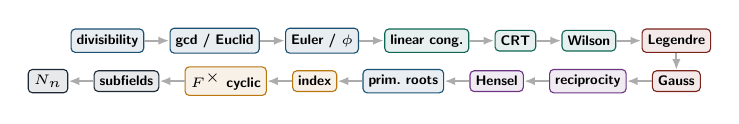
\begin{tikzpicture}[
  font=\sffamily\tiny,
  node distance=2.2mm and 3.2mm,
  n/.style={draw=#1, fill=#1!10, rounded corners=1.5pt, inner sep=2pt, font=\sffamily\tiny\bfseries},
  a/.style={-{Latex[length=1.4mm]}, gray!65, thick}
]
\node[n=L2] (1) {divisibility};
\node[n=L2, right=of 1] (2) {gcd / Euclid};
\node[n=L2, right=of 2] (3) {Euler / $\phi$};
\node[n=L3, right=of 3] (4) {linear cong.};
\node[n=L3, right=of 4] (5) {CRT};
\node[n=L3, right=of 5] (6) {Wilson};
\node[n=L4, right=of 6] (7) {Legendre};
\node[n=L4, below=of 7] (8) {Gauss};
\node[n=L5, left=of 8] (9) {reciprocity};
\node[n=L5, left=of 9] (10) {Hensel};
\node[n=L6, left=of 10] (11) {prim.\ roots};
\node[n=L7, left=of 11] (12) {index};
\node[n=L7, left=of 12] (13) {$F^\times$ cyclic};
\node[n=L8, left=of 13] (14) {subfields};
\node[n=L8, left=of 14] (15) {$N_n$};

\foreach \x/\y in {1/2,2/3,3/4,4/5,5/6,6/7,7/8,8/9,9/10,10/11,11/12,12/13,13/14,14/15}
  \draw[a] (\x) -- (\y);
\end{tikzpicture}
\end{center}

\end{document}
